\documentclass{article}
\usepackage[spanish,activeacute]{babel}
\usepackage{changepage}
\usepackage[utf8]{inputenc}
\usepackage{graphicx}
\usepackage{color}
\usepackage[dvipsnames]{xcolor}
\usepackage[labelformat=empty]{caption}
\newenvironment{allintypewriter}{\ttfamily}{\par}


%% Datos del documento
\title{Reto 4.}
\author{Mario Román}


%% Cuerpo del documento
\begin{document}

\maketitle

\section {Codificación de un árbol binario.}
\subsection {Consideraciones previas}

Vamos a intentar codificar un árbol binario con la menor cantidad de información posible, esto es,
con el menor número de bits que podamos. La condición que debe tener una codificación es que sea unívoca,
y nos permita recuperar el árbol de manera única una vez codificado.

Queremos codificar un árbol binario genérico, que puede contener como datos cualesquiera etiquetas. La codificación
de estos datos, que podrían tener diversa naturaleza (las etiquetas podrían ser enteros, cadenas, o incluso listas de colas de pilas de árboles de booleanos),
se debería considerar aparte. Dado un árbol, tomaremos su preorden y lo almacenaremos en un vector. Este vector contiene la información de las etiquetas del árbol e, 
implícitamente, el número de nodos que tiene.

\begin{figure}[ht!]
\centering
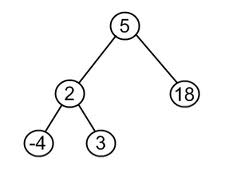
\includegraphics[width=50mm]{ejemplo.jpeg}
\caption{Árbol de ejemplo.}
\label{overflow}
\end{figure}

En el ejemplo, de $5$ nodos, codificaríamos:
\begin{adjustwidth}{2cm}{}
 $[5,2,-4,3,18]$
\end{adjustwidth}
 
Es decir, que nuestro problema se centra en codificar la estructura, el esqueleto de un árbol binario.
Consideramos que las etiquetas se codifican aparte.

Intentaremos conseguir la mejor codificación posible de la estructura de un árbol de $n$ nodos creando una
función biyectiva entre árboles binarios y números naturales; y codificando el número natural que nos dé la biyección.


\subsection {Orden total entre árboles.}

La herramienta que usaremos para hacer esto posible es la definición de un orden total entre esqueletos de árboles.
Abusaremos del lenguaje llamándolos árboles, pero nótese que no tendrán etiquetas.

Definimos un esqueleto de árbol binario con la forma $A = (A_i,A_d)$, es decir, constando sólo de un
un subesqueleto izquierdo, y un subesqueleto derecho; o como un esqueleto vacío $A = nulo$. Nótese que la definición
es igual a la de los árboles binarios pero sin etiqueta.\\

Ahora definimos la relación de orden como sigue:
\begin{adjustwidth}{2cm}{}
 $\qquad A = (A_i,A_d) \leq B = (B_i,B_d)$ 
\end{adjustwidth}
 Si se cumple: 
 \begin{adjustwidth}{2cm}{}
 $\qquad nodos totales(A) <  nodos totales(B)$ 
 \end{adjustwidth}
 O si tienen el mismo número de nodos pero: 
 \begin{adjustwidth}{2cm}{}
 $\qquad A_d < B_d$ 
 \end{adjustwidth}
 O si tienen el mismo subárbol derecho pero: 
 \begin{adjustwidth}{2cm}{}
 $\qquad A_i \leq B_i$ 
\end{adjustwidth}
Es decir, primero comparamos el número de nodos, luego el subárbol derecho, y como último criterio, comparamos el subárbol izquierdo.\\

Claramente es una relación de orden. Es antisimétrica porque dos árboles con mismos nodos y subárboles deben ser iguales.
Es transitiva por ser composición de varias relaciones de orden. Y es trivialmente reflexiva. \\

Pero además, es una relación de orden total. Trivialmente lo es para árboles de un nodo. Y, por inducción sobre el número de nodos lo demostramos para árboles de $n$ nodos: \\
\indent Que sea relación de orden total para árboles de menos $n$ nodos fuerza a que deba darse $A_i \leq B_i$ o $A_i \leq B_i$, ya que el subárbol izquierdo 
tiene menos de $n$ nodos, y por tanto, al menos la tercera condición debe cumplirse en alguno de los dos sentidos.


\subsection {Convertir árboles en números.}

Ahora usaremos que existen $\frac{1}{n+1} {2n \choose n}$ árboles binarios de $n$ nodos. Llamamos $A_n$ al conjunto de esqueletos de árboles binarios
de $n$ nodos, y sabemos que:
\begin{adjustwidth}{2cm}{}
$\#A_n = \frac{1}{n+1} {2n \choose n} = C_n$ \\
\end{adjustwidth}

Definimos la siguiente función:
\begin{adjustwidth}{2cm}{}
 $f : A_n \longrightarrow \{1,2,\dots,C_n\}$ 
\end{adjustwidth}
Como la única biyección estrictamente creciente entre los dos conjuntos. Es decir, la única que cumple:
\begin{adjustwidth}{2cm}{}
 $\displaystyle \forall X,Y \in A_n : X \leq Y \Longleftrightarrow f(X) \leq f(Y)$
\end{adjustwidth}
Es resultado conocido que entre dos conjuntos con el mismo cardinal y con dos relaciones totales de orden,
existe una única aplicación biyectiva creciente. \\

Una forma práctica de hallar la imagen de un árbol por $f$ es generar la lista ordenada de posibles estructuras de árboles de $n$ y
realizar una búsqueda binaria sobre ella (aprovechando que hemos definido una relación de orden) hasta encontrar el índice
de un árbol que coincida con el árbol buscado. Esa es su codificación. 
 Lo que estamos haciendo, expuesto de otra forma, es contar todos los posibles árboles, ordenarlos e irles asignando su número según el orden.
 En la implementación se concretan estos detalles.\\

Otra forma, que no se desarrolla aquí, mucho más
eficiente, es la de relacionar el valor de $f$ para un árbol de $n$ nodos, con los valores de $f(A_i)$ y $f(A_d)$, que pueden buscarse inductivamente.



\subsection {Palabras binarias y codificación.}
La codificación de un árbol binario $A$ se define entonces como un vector con sus elementos en preorden, que nos da el número de nodos
del árbol, y el número $f(A)$ escrito como una palabra binaria. Es decir, los números pueden escribirse con los mínimos bits posibles siguiendo este patrón.
\begin{adjustwidth}{2cm}{}
 $0 \rightarrow ""$\\
 $1 \rightarrow "0"$ \\
 $2 \rightarrow "1"$ \\
 $3 \rightarrow "00"$ \\
 $4 \rightarrow "10"$ \\
 $5 \rightarrow "01"$ \\
 $6 \rightarrow "11"$ \\
 $7 \rightarrow "000"$ \\
 $8 \rightarrow "100"$ \\
 $\dots$ \\
\end{adjustwidth}

Es decir, guardamos por un lado los nodos, y por otro escribimos el número que determina unívocamente el árbol por la función $f$.

Por ejemplo, vamos a escribir los árboles de tres nodos ordenados: \\
\begin{figure}[ht!]
\centering
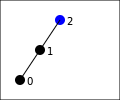
\includegraphics[width=20mm]{0.png}
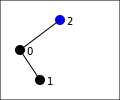
\includegraphics[width=20mm]{1.png}
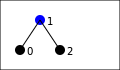
\includegraphics[width=20mm]{2.png}
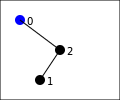
\includegraphics[width=20mm]{3.png}
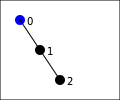
\includegraphics[width=20mm]{4.png}
\caption{""}
\label{overflow}
\end{figure}


Donde las estructuras de los árboles tendrán, respectivamente, las codificaciones siguientes:
%\begin{adjustwidth}{2cm}{}
 $"", "0", "1", "00", "10"$
%\end{adjustwidth}
\newpage

Un ejemplo con el árbol inicial, un árbol con nodos significativos y no sólo estructura, es el siguiente:
\begin{figure}[htbp]
\centering
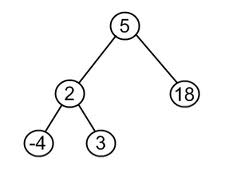
\includegraphics[width=50mm]{ejemplo.jpeg}
\caption{Árbol de ejemplo, de nuevo.}
\label{overflow}
\end{figure}

Su codificación será: $([5,2,-4,3,18],"1010")$.
Ya que es el número $25$ entre los posibles árboles de $5$ nodos, y la codificación de $25$ es $"1010"$.
La otra parte de la codificación es el inorden de los nodos.



\subsection {Tamaño de la codificación.}

Ahora vamos a medir cuánto ocupa la codificación de un árbol de $n$ nodos.
Es claro que las etiquetas, si son de tipo $Type$, ocuparán en disco:
\begin{adjustwidth}{2cm}{}
 $n * sizeof(Type)$
\end{adjustwidth}
Quizá algo más si contamos un caracter terminador o uno que indique cuántos elementos hay.\\

La parte más interesante para medir será cuánto ocupa la codificación de la estructura.
Tenemos que una palabra binaria de, como máximo, $m$ bits puede codificar:
\begin{adjustwidth}{2cm}{}
 $\displaystyle \sum_{k=0}^{m} 2^{k} = 2^{m+1} - 1$
\end{adjustwidth}
Donde cada sumando representa las $2^b$ cadenas posibles con $b$ bits.\\

Pero tenemos por otro lado que hay $\frac{1}{n+1} {2n \choose n}$ posibles árboles, si queremos saber
cuánto espacio necesitaremos para codificarlos, resolvemos:
\begin{adjustwidth}{2cm}{}
 $\displaystyle 2^{m_n+1} - 1 = \frac{1}{n+1} {2n \choose n};$ \\
 $\displaystyle m_n = \left\lceil log_2 \left( \frac{1}{n+1} {2n \choose n} + 1 \right) - 1 \right\rceil;$ \\
\end{adjustwidth}

Este será el espacio que usemos. Asintóticamente, sabemos que la función de los números de Catalan crece como:
\begin{adjustwidth}{2cm}{}
 $\displaystyle C_n \sim \frac{4^n}{n^{3/2}\sqrt\pi}$
\end{adjustwidth}
Por lo que la función en conjunto se aproximará a:
\begin{adjustwidth}{2cm}{}
 $\displaystyle m_n \sim \left\lceil log_2 \left( \frac{4^n}{n^{3/2}\sqrt\pi} + 1 \right) - 1 \right\rceil \sim 2n - log_2\left(n^{3/2}\sqrt\pi\right) \sim 2n - \frac{3}{2}log_2(n)$
\end{adjustwidth}
Que aunque siga siendo $O(n)$, es menor que la que use invariablemente $2n$, a pesar de que se aproxime asintóticamente a ella.

\subsection {Mejor codificación.}

Toda codificación de los esqueletos de árboles binarios como palabras binarias debe ser inyectiva, para permitir que pueda recuperarse de ella el árbol binario original de manera unívoca, y
sin dar lugar a pérdida de información. Por tanto, será una biyección con su conjunto imagen. El cardinal de la imagen de una biyección debe tener al menos el mismo número de elementos
que el cardinal del conjunto de definición, en este caso, para $n$ nodos, $C_n$ elementos.

La función aquí presentada alcanza el mínimo especificado en esa cota, así que cualquier otra codificación debe usar los mismos o más elementos que ella. Es decir, cualquier otra
codificación llevará árboles en palabras binarias que como poco, alcanzarán las $C_n$ palabras distintas, y necesitará usar, como poco, tantos bits como en este caso.\\

Podríamos obtener mejoras en la codificación de las etiquetas, o si tenemos una restricción sobre ellas, o si nos preocupamos en codificar mejor los árboles más comunes para mejorar el caso medio;
pero en las condiciones que hemos fijado, tenemos la mínima codificación posible.


\subsection {Implementación.}

Se presenta una implementación de la codificación en lenguaje de programación Haskell. Usamos por comodidad este lenguaje porque nos permite hacer definiciones más
concisas de los árboles y las funciones sobre ellos que C++, a pesar de que perdemos mucha eficiencia. Nótese que no se ha hecho referencia a la eficiencia del algoritmo en
ningún momento. Sólo nos interesa obtener la minima codificación, y los algoritmos usados para comprimir y descomprimir serán muy ineficientes.\\

Al final de la implementación se da un ejemplo de uso.\\

% Generator: GNU source-highlight, by Lorenzo Bettini, http://www.gnu.org/software/src-highlite

\begin{allintypewriter}
 



\noindent
\mbox{}\textbf{\textcolor{Blue}{import}}\ Data\textcolor{BrickRed}{.}\textcolor{ForestGreen}{List} \\
\mbox{}\textbf{\textcolor{Blue}{import}}\ Data\textcolor{BrickRed}{.}\textcolor{ForestGreen}{Maybe} \\
\mbox{}\textbf{\textcolor{Blue}{import}}\ Data\textcolor{BrickRed}{.}\textcolor{ForestGreen}{Char} \\
\mbox{} \\
\mbox{}\textit{\textcolor{Brown}{\{-\ 1a\ Parte:\ Esqueletos\ de\ Arbol\ -\}}} \\
\mbox{} \\
\mbox{}\textit{\textcolor{Brown}{\{-\ }} \\
\mbox{}\textit{\textcolor{Brown}{\ \ \ Definimos\ lo\ que\ sera\ el\ esqueleto\ de\ un\ arbol,\ }} \\
\mbox{}\textit{\textcolor{Brown}{\ es\ decir,\ un\ arbol\ sin\ etiquetas\ en\ los\ nodos,\ un\ arbol\ binario\ puro,}} \\
\mbox{}\textit{\textcolor{Brown}{\ considerando\ solo\ su\ estructura.}} \\
\mbox{} \\
\mbox{}\textit{\textcolor{Brown}{\ \ \ Un\ esqueleto\ se\ define\ como\ un\ esqueleto\ vacio\ o\ como\ un\ punto\ (nodo)}} \\
\mbox{}\textit{\textcolor{Brown}{\ del\ que\ salen\ dos\ esqueletos\ de\ arbol.}} \\
\mbox{}\textit{\textcolor{Brown}{-\}}} \\
\mbox{}\textbf{\textcolor{Blue}{data}}\ \textcolor{ForestGreen}{EsqArbol}\ \textcolor{BrickRed}{=}\ \textcolor{ForestGreen}{EsqVacio} \\
\mbox{}\ \ \ \ \ \ \ \ \ \ \ \ \ \ \textcolor{BrickRed}{$|$}\ \textcolor{ForestGreen}{Punto}\ \textcolor{BrickRed}{(}\textcolor{ForestGreen}{EsqArbol}\textcolor{BrickRed}{)}\ \textcolor{BrickRed}{(}\textcolor{ForestGreen}{EsqArbol}\textcolor{BrickRed}{)} \\
\mbox{}\ \ \ \ \ \ \ \ \ \ \ \ \ \ \ \ \textbf{\textcolor{Blue}{deriving}}\ \textcolor{BrickRed}{(}\textcolor{ForestGreen}{Show}\textcolor{BrickRed}{,}\ \textcolor{ForestGreen}{Eq}\textcolor{BrickRed}{)} \\
\mbox{} \\
\mbox{} \\
\mbox{}\textit{\textcolor{Brown}{\{-}} \\
\mbox{}\textit{\textcolor{Brown}{\ \ \ Definimos\ una\ funcion\ recursiva\ trivial\ para\ contar\ nodos\ de\ un\ esqueleto.}} \\
\mbox{}\textit{\textcolor{Brown}{\ Creamos\ una\ funcion\ que\ crea\ todos\ los\ posibles\ esqueletos\ de\ n\ nodos.\ Para\ ello,}} \\
\mbox{}\textit{\textcolor{Brown}{\ en\ el\ caso\ inductivo,\ crea,\ para\ todo\ i\ en\ el\ rango\ [0,...,n-1]\ todos\ los\ posibles\ }} \\
\mbox{}\textit{\textcolor{Brown}{\ arboles\ con\ i\ nodos\ a\ la\ izquierda\ y\ todos\ los\ posibles\ con\ n-1-i\ nodos\ a\ la\ derecha.}} \\
\mbox{}\textit{\textcolor{Brown}{\ -\}}} \\
\mbox{}nodos\ \textcolor{BrickRed}{::}\ \textcolor{ForestGreen}{EsqArbol}\ \textcolor{BrickRed}{-\textgreater{}}\ \textcolor{ForestGreen}{Int}\  \\
\mbox{}nodos\ \textcolor{ForestGreen}{EsqVacio}\ \textcolor{BrickRed}{=}\ \textcolor{Purple}{0} \\
\mbox{}nodos\ \textcolor{BrickRed}{(}\textcolor{ForestGreen}{Punto}\ a\ b\textcolor{BrickRed}{)}\ \textcolor{BrickRed}{=}\ \textcolor{Purple}{1}\ \textcolor{BrickRed}{+}\ \textcolor{BrickRed}{(}nodos\ a\textcolor{BrickRed}{)}\ \textcolor{BrickRed}{+}\ \textcolor{BrickRed}{(}nodos\ b\textcolor{BrickRed}{)} \\
\mbox{} \\
\mbox{}arbolesNodos\ \textcolor{BrickRed}{::}\ \textcolor{ForestGreen}{Int}\ \textcolor{BrickRed}{-\textgreater{}}\ \textcolor{BrickRed}{[}\textcolor{ForestGreen}{EsqArbol}\textcolor{BrickRed}{]} \\
\mbox{}arbolesNodos\ \textcolor{Purple}{0}\ \textcolor{BrickRed}{=}\ \textcolor{BrickRed}{[}\textcolor{ForestGreen}{EsqVacio}\textcolor{BrickRed}{]} \\
\mbox{}arbolesNodos\ \textcolor{Purple}{1}\ \textcolor{BrickRed}{=}\ \textcolor{BrickRed}{[(}\textcolor{ForestGreen}{Punto}\ \textcolor{ForestGreen}{EsqVacio}\ \textcolor{ForestGreen}{EsqVacio}\textcolor{BrickRed}{)]} \\
\mbox{}arbolesNodos\ n\ \textcolor{BrickRed}{=}\ concat\ \textcolor{BrickRed}{[[}\textcolor{ForestGreen}{Punto}\ x\ y\ \textcolor{BrickRed}{$|$}\ y\ \textcolor{BrickRed}{\textless{}-}\ arbolesNodos\ \textcolor{BrickRed}{(}n\textcolor{BrickRed}{-}\textcolor{Purple}{1}\textcolor{BrickRed}{-}i\textcolor{BrickRed}{),}\ x\ \textcolor{BrickRed}{\textless{}-}\ arbolesNodos\ \textcolor{BrickRed}{(}i\textcolor{BrickRed}{)]}\ \textcolor{BrickRed}{$|$}\ i\ \textcolor{BrickRed}{\textless{}-}\ \textcolor{BrickRed}{[}\textcolor{Purple}{0}\textcolor{BrickRed}{..}n\textcolor{BrickRed}{-}\textcolor{Purple}{1}\textcolor{BrickRed}{]]} \\
\mbox{} \\
\mbox{}\textit{\textcolor{Brown}{\{-\ Como\ curiosidad,\ podemos\ notar\ que\ hay\ C$\_$n\ arboles\ de\ n\ nodos,\ donde\ C$\_$n\ es\ el\ }} \\
\mbox{}\textit{\textcolor{Brown}{\ enesimo\ numero\ de\ Catalan.\ La\ longitud\ de\ la\ lista\ creadas\ por\ "{}arbolesNodos\ n"{}\ es\ C$\_$n\ -\}}} \\
\mbox{} \\
\mbox{} \\
\mbox{}\textit{\textcolor{Brown}{\{-\ }} \\
\mbox{}\textit{\textcolor{Brown}{\ \ \ Ahora\ vamos\ a\ codificar\ un\ esqueleto\ binario.\ Para\ ello,\ asignamos\ a\ cada\ arbol}} \\
\mbox{}\textit{\textcolor{Brown}{\ su\ posicion\ en\ la\ lista\ de\ arboles\ generados,\ y\ escribimos\ el\ numero\ como\ palabra\ binaria.}} \\
\mbox{} \\
\mbox{}\textit{\textcolor{Brown}{\ \ \ Para\ pasar\ a\ binario,\ intentamos\ aprovechar\ al\ maximo\ el\ espacio,\ para\ ello\ usamos\ todas}} \\
\mbox{}\textit{\textcolor{Brown}{\ las\ palabras\ binarias\ posibles.\ Es\ decir,\ transformamos:}} \\
\mbox{}\textit{\textcolor{Brown}{\ \ \ \ 0\ -\textgreater{}\ $\_$}} \\
\mbox{}\textit{\textcolor{Brown}{\ \ \ \ 1\ -\textgreater{}\ 0}} \\
\mbox{}\textit{\textcolor{Brown}{\ \ \ \ 2\ -\textgreater{}\ 1}} \\
\mbox{}\textit{\textcolor{Brown}{\ \ \ \ 3\ -\textgreater{}\ 00}} \\
\mbox{}\textit{\textcolor{Brown}{\ \ \ \ 4\ -\textgreater{}\ 01}} \\
\mbox{}\textit{\textcolor{Brown}{\ \ \ Adjuntamos\ ademas\ otra\ funcion\ para\ pasarlo\ a\ una\ cadena\ legible\ de\ texto}} \\
\mbox{}\textit{\textcolor{Brown}{\ -\}}} \\
\mbox{}aBinario\ \textcolor{BrickRed}{::}\ \textcolor{ForestGreen}{Int}\ \textcolor{BrickRed}{-\textgreater{}}\ \textcolor{BrickRed}{[}\textcolor{ForestGreen}{Int}\textcolor{BrickRed}{]} \\
\mbox{}aBinario\ \textcolor{Purple}{0}\ \textcolor{BrickRed}{=}\ \textcolor{BrickRed}{[]} \\
\mbox{}aBinario\ n\ \textcolor{BrickRed}{=}\ r\ \textcolor{BrickRed}{:}\ aBinario\ q \\
\mbox{}\ \ \textbf{\textcolor{Blue}{where}}\ \textcolor{BrickRed}{(}q\textcolor{BrickRed}{,}r\textcolor{BrickRed}{)}\ \textcolor{BrickRed}{=}\ divMod\ \textcolor{BrickRed}{(}n\textcolor{BrickRed}{-}\textcolor{Purple}{1}\textcolor{BrickRed}{)}\ \textcolor{Purple}{2} \\
\mbox{} \\
\mbox{}binarioLegible\ \textcolor{BrickRed}{::}\ \textcolor{ForestGreen}{Int}\ \textcolor{BrickRed}{-\textgreater{}}\ \textcolor{ForestGreen}{String} \\
\mbox{}binarioLegible\ x\ \textcolor{BrickRed}{=}\ map\ intToDigit\ \textcolor{BrickRed}{\$}\ reverse\ \textcolor{BrickRed}{\$}\ aBinario\ x \\
\mbox{} \\
\mbox{}codifica\ \textcolor{BrickRed}{::}\ \textcolor{ForestGreen}{EsqArbol}\ \textcolor{BrickRed}{-\textgreater{}}\ \textcolor{ForestGreen}{Int} \\
\mbox{}codifica\ x\ \textcolor{BrickRed}{=}\ fromJust\ \textcolor{BrickRed}{\$}\ elemIndex\ x\ \textcolor{BrickRed}{(}arbolesNodos\ len\textcolor{BrickRed}{)} \\
\mbox{}\ \ \textbf{\textcolor{Blue}{where}}\ len\ \textcolor{BrickRed}{=}\ nodos\ x \\
\mbox{} \\
\mbox{}codificaLegible\ \textcolor{BrickRed}{::}\ \textcolor{ForestGreen}{EsqArbol}\ \textcolor{BrickRed}{-\textgreater{}}\ \textcolor{ForestGreen}{String} \\
\mbox{}codificaLegible\ x\ \textcolor{BrickRed}{=}\ binarioLegible\ \textcolor{BrickRed}{\$}\ codifica\ x \\
\mbox{} \\
\mbox{} \\
\mbox{}\textit{\textcolor{Brown}{\{-\ }} \\
\mbox{}\textit{\textcolor{Brown}{\ \ \ Por\ ultimo,\ implementamos\ la\ decodificacion.\ }} \\
\mbox{}\textit{\textcolor{Brown}{\ Notese\ que\ aqui\ debe\ conocerse\ el\ numero\ de\ nodos.}} \\
\mbox{}\textit{\textcolor{Brown}{-\}}} \\
\mbox{}aNatural\ \textcolor{BrickRed}{::}\ \textcolor{BrickRed}{[}\textcolor{ForestGreen}{Int}\textcolor{BrickRed}{]}\ \textcolor{BrickRed}{-\textgreater{}}\ \textcolor{ForestGreen}{Int} \\
\mbox{}aNatural\ \textcolor{BrickRed}{[]}\ \textcolor{BrickRed}{=}\ \textcolor{Purple}{0} \\
\mbox{}aNatural\ \textcolor{BrickRed}{(}x\textcolor{BrickRed}{:}xs\textcolor{BrickRed}{)}\ \textcolor{BrickRed}{=}\ \textcolor{Purple}{2}\textcolor{BrickRed}{*(}aNatural\ xs\textcolor{BrickRed}{)}\ \textcolor{BrickRed}{+}\ x\ \textcolor{BrickRed}{+}\ \textcolor{Purple}{1} \\
\mbox{} \\
\mbox{}decodifica\ \textcolor{BrickRed}{::}\ \textcolor{ForestGreen}{Int}\ \textcolor{BrickRed}{-\textgreater{}}\ \textcolor{ForestGreen}{Int}\ \textcolor{BrickRed}{-\textgreater{}}\ \textcolor{ForestGreen}{EsqArbol} \\
\mbox{}decodifica\ x\ nodos\ \textcolor{BrickRed}{=}\ \textcolor{BrickRed}{(}arbolesNodos\ nodos\textcolor{BrickRed}{)}\ \textcolor{BrickRed}{!!}\ x\  \\
\mbox{} \\
\mbox{}decodificaBinario\ \textcolor{BrickRed}{::}\ \textcolor{BrickRed}{[}\textcolor{ForestGreen}{Int}\textcolor{BrickRed}{]}\ \textcolor{BrickRed}{-\textgreater{}}\ \textcolor{ForestGreen}{Int}\ \textcolor{BrickRed}{-\textgreater{}}\ \textcolor{ForestGreen}{EsqArbol} \\
\mbox{}decodificaBinario\ xs\ nodos\ \textcolor{BrickRed}{=}\ decodifica\ \textcolor{BrickRed}{(}aNatural\ xs\textcolor{BrickRed}{)}\ nodos\ \  \\
\mbox{} \\
\mbox{}decodificaLegible\ \textcolor{BrickRed}{::}\ \textcolor{ForestGreen}{String}\ \textcolor{BrickRed}{-\textgreater{}}\ \textcolor{ForestGreen}{Int}\ \textcolor{BrickRed}{-\textgreater{}}\ \textcolor{ForestGreen}{EsqArbol} \\
\mbox{}decodificaLegible\ s\ nodos\ \textcolor{BrickRed}{=}\ decodificaBinario\ \textcolor{BrickRed}{(}reverse\ \textcolor{BrickRed}{(}map\ digitToInt\ \textcolor{BrickRed}{\$}\ s\textcolor{BrickRed}{))}\ nodos \\
\mbox{} \\
\mbox{}\ \  \\
\mbox{} \\
\mbox{} \\
\mbox{}\textit{\textcolor{Brown}{\{-\ 2a\ Parte:\ Arboles\ de\ verdad.\ -\}}} \\
\mbox{} \\
\mbox{}\textit{\textcolor{Brown}{\{-}} \\
\mbox{}\textit{\textcolor{Brown}{\ \ Para\ ver\ la\ aplicacion\ real\ del\ algoritmo,\ vamos\ a\ escribir\ arboles}} \\
\mbox{}\textit{\textcolor{Brown}{\ de\ verdad\ y\ a\ codificarlos.\ Definimos\ un\ arbol\ de\ manera\ parecida\ al\ esqueleto.}} \\
\mbox{}\textit{\textcolor{Brown}{\ Como\ diferencia,\ ahora\ permitimos\ que\ la\ etiqueta\ contenga\ un\ dato\ de\ tipo\ a.}} \\
\mbox{}\textit{\textcolor{Brown}{-\}}} \\
\mbox{}\textbf{\textcolor{Blue}{data}}\ \textcolor{ForestGreen}{Arbol}\ a\ \textcolor{BrickRed}{=}\ \textcolor{ForestGreen}{ArbolVacio}\  \\
\mbox{}\ \ \ \ \ \ \ \ \ \ \ \ \textcolor{BrickRed}{$|$}\ \textcolor{ForestGreen}{Nodo}\ a\ \textcolor{BrickRed}{(}\textcolor{ForestGreen}{Arbol}\ a\textcolor{BrickRed}{)}\ \textcolor{BrickRed}{(}\textcolor{ForestGreen}{Arbol}\ a\textcolor{BrickRed}{)} \\
\mbox{}\ \ \ \ \ \ \ \ \ \ \ \ \textbf{\textcolor{Blue}{deriving}}\ \textcolor{BrickRed}{(}\textcolor{ForestGreen}{Show}\textcolor{BrickRed}{,}\ \textcolor{ForestGreen}{Eq}\textcolor{BrickRed}{)} \\
\mbox{} \\
\mbox{} \\
\mbox{}\textit{\textcolor{Brown}{\{-}} \\
\mbox{}\textit{\textcolor{Brown}{\ \ \ Codifica\ un\ arbol\ binario.}} \\
\mbox{}\textit{\textcolor{Brown}{\ \ Para\ ello,\ toma\ sus\ elementos\ y\ los\ guarda,\ por\ otro\ lado,\ lo\ transforma\ en\ esqueleto.\ }} \\
\mbox{}\textit{\textcolor{Brown}{\ \ La\ codificacion\ son\ sus\ elementos,\ implicita\ su\ longitud,\ y\ la\ codificacion\ binaria\ del\ esqueleto.}} \\
\mbox{}\textit{\textcolor{Brown}{-\}}} \\
\mbox{}transformaEsqueleto\ \textcolor{BrickRed}{::}\ \textcolor{ForestGreen}{Arbol}\ a\ \textcolor{BrickRed}{-\textgreater{}}\ \textcolor{ForestGreen}{EsqArbol} \\
\mbox{}transformaEsqueleto\ \textcolor{ForestGreen}{ArbolVacio}\ \textcolor{BrickRed}{=}\ \textcolor{ForestGreen}{EsqVacio} \\
\mbox{}transformaEsqueleto\ \textcolor{BrickRed}{(}\textcolor{ForestGreen}{Nodo}\ \textbf{\textcolor{Blue}{$\_$}}\ a\ b\textcolor{BrickRed}{)}\ \textcolor{BrickRed}{=}\ \textcolor{BrickRed}{(}\textcolor{ForestGreen}{Punto}\ \textcolor{BrickRed}{(}transformaEsqueleto\ a\textcolor{BrickRed}{)}\ \textcolor{BrickRed}{(}transformaEsqueleto\ b\textcolor{BrickRed}{))} \\
\mbox{} \\
\mbox{}preorden\ \textcolor{BrickRed}{::}\ \textcolor{ForestGreen}{Arbol}\ a\ \textcolor{BrickRed}{-\textgreater{}}\ \textcolor{BrickRed}{[}a\textcolor{BrickRed}{]} \\
\mbox{}preorden\ \textcolor{ForestGreen}{ArbolVacio}\ \textcolor{BrickRed}{=}\ \textcolor{BrickRed}{[]} \\
\mbox{}preorden\ \textcolor{BrickRed}{(}\textcolor{ForestGreen}{Nodo}\ x\ a\ b\textcolor{BrickRed}{)}\ \textcolor{BrickRed}{=}\ x\ \textcolor{BrickRed}{:}\ \textcolor{BrickRed}{((}preorden\ a\textcolor{BrickRed}{)}\ \textcolor{BrickRed}{++}\ \textcolor{BrickRed}{(}preorden\ b\textcolor{BrickRed}{))} \\
\mbox{} \\
\mbox{}codificaArbol\ \textcolor{BrickRed}{::}\ \textcolor{ForestGreen}{Arbol}\ a\ \textcolor{BrickRed}{-\textgreater{}}\ \textcolor{BrickRed}{([}a\textcolor{BrickRed}{],}\ \textcolor{ForestGreen}{String}\textcolor{BrickRed}{)} \\
\mbox{}codificaArbol\ x\ \textcolor{BrickRed}{=}\ \textcolor{BrickRed}{(}preorden\ x\textcolor{BrickRed}{,}\ codificaLegible\textcolor{BrickRed}{.}transformaEsqueleto\ \textcolor{BrickRed}{\$}\ x\textcolor{BrickRed}{)} \\
\mbox{} \\
\mbox{} \\
\mbox{}\textit{\textcolor{Brown}{\{-}} \\
\mbox{}\textit{\textcolor{Brown}{\ \ \ Decodifica\ un\ arbol\ binario.}} \\
\mbox{}\textit{\textcolor{Brown}{\ Para\ ello,\ decodifica\ el\ esqueleto\ del\ arbol\ }} \\
\mbox{}\textit{\textcolor{Brown}{\ y\ rellena\ el\ esqueleto\ con\ los\ elementos\ del\ preorden.}} \\
\mbox{}\textit{\textcolor{Brown}{-\}}} \\
\mbox{} \\
\mbox{}rellenaEsqueleto\ \textcolor{BrickRed}{::}\ \textcolor{ForestGreen}{EsqArbol}\ \textcolor{BrickRed}{-\textgreater{}}\ \textcolor{BrickRed}{[}a\textcolor{BrickRed}{]}\ \textcolor{BrickRed}{-\textgreater{}}\ \textcolor{ForestGreen}{Arbol}\ a \\
\mbox{}rellenaEsqueleto\ \textcolor{ForestGreen}{EsqVacio}\ \textbf{\textcolor{Blue}{$\_$}}\ \textcolor{BrickRed}{=}\ \textcolor{ForestGreen}{ArbolVacio} \\
\mbox{}rellenaEsqueleto\ \textbf{\textcolor{Blue}{$\_$}}\ \textcolor{BrickRed}{[]}\ \textcolor{BrickRed}{=}\ \textcolor{ForestGreen}{ArbolVacio} \\
\mbox{}rellenaEsqueleto\ \textcolor{BrickRed}{(}\textcolor{ForestGreen}{Punto}\ u\ v\textcolor{BrickRed}{)}\ \textcolor{BrickRed}{(}x\textcolor{BrickRed}{:}xs\textcolor{BrickRed}{)}\ \textcolor{BrickRed}{=}\ \textcolor{BrickRed}{(}\textcolor{ForestGreen}{Nodo}\ x\ subIzquierdo\ subDerecho\textcolor{BrickRed}{)} \\
\mbox{}\ \ \textbf{\textcolor{Blue}{where}}\ \textcolor{BrickRed}{(}parteIzquierda\textcolor{BrickRed}{,}\ parteDerecha\textcolor{BrickRed}{)}\ \textcolor{BrickRed}{=}\ splitAt\ \textcolor{BrickRed}{(}nodos\ u\textcolor{BrickRed}{)}\ xs \\
\mbox{}\ \ \ \ \ \ \ \ subIzquierdo\ \textcolor{BrickRed}{=}\ rellenaEsqueleto\ u\ parteIzquierda \\
\mbox{}\ \ \ \ \ \ \ \ subDerecho\ \ \ \textcolor{BrickRed}{=}\ rellenaEsqueleto\ v\ parteDerecha \\
\mbox{} \\
\mbox{}decodificaArbol\ \textcolor{BrickRed}{::}\ \textcolor{BrickRed}{([}a\textcolor{BrickRed}{],}\ \textcolor{ForestGreen}{String}\textcolor{BrickRed}{)}\ \textcolor{BrickRed}{-\textgreater{}}\ \textcolor{ForestGreen}{Arbol}\ a \\
\mbox{}decodificaArbol\ \textcolor{BrickRed}{(}datos\textcolor{BrickRed}{,}\ codificado\textcolor{BrickRed}{)}\ \textcolor{BrickRed}{=}\ rellenaEsqueleto\ \textcolor{BrickRed}{(}decodificaLegible\ codificado\ nodos\textcolor{BrickRed}{)}\ datos \\
\mbox{}\ \ \textbf{\textcolor{Blue}{where}}\ nodos\ \textcolor{BrickRed}{=}\ length\ datos \\
\mbox{}\ \ \ \ \ \ \ \  \\
\mbox{} \\
\mbox{} \\
\mbox{}\textit{\textcolor{Brown}{\{-\ 3a\ Parte:\ Funciones\ auxiliares.\ -\}}} \\
\mbox{}\textit{\textcolor{Brown}{\{-}} \\
\mbox{}\textit{\textcolor{Brown}{\ \ Para\ poder\ aprovechar\ la\ codificacion\ creada,\ se\ presentan\ funciones\ auxiliares\ que}} \\
\mbox{}\textit{\textcolor{Brown}{\ faciliten\ ejemplos\ de\ uso.}} \\
\mbox{}\textit{\textcolor{Brown}{-\}}} \\
\mbox{} \\
\mbox{}insercionEnArbol\ \textcolor{BrickRed}{::}\ \textcolor{BrickRed}{(}\textcolor{ForestGreen}{Ord}\ a\textcolor{BrickRed}{)}\ \textcolor{BrickRed}{=\textgreater{}}\ a\ \textcolor{BrickRed}{-\textgreater{}}\ \textcolor{ForestGreen}{Arbol}\ a\ \textcolor{BrickRed}{-\textgreater{}}\ \textcolor{ForestGreen}{Arbol}\ a \\
\mbox{}insercionEnArbol\ x\ \textcolor{ForestGreen}{ArbolVacio}\ \textcolor{BrickRed}{=}\ \textcolor{BrickRed}{(}\textcolor{ForestGreen}{Nodo}\ x\ \textcolor{ForestGreen}{ArbolVacio}\ \textcolor{ForestGreen}{ArbolVacio}\textcolor{BrickRed}{)} \\
\mbox{}insercionEnArbol\ x\ \textcolor{BrickRed}{(}\textcolor{ForestGreen}{Nodo}\ a\ izq\ der\textcolor{BrickRed}{)} \\
\mbox{}\ \ \textcolor{BrickRed}{$|$}\ x\ \textcolor{BrickRed}{\textless{}=}\ a\ \ \textcolor{BrickRed}{=}\ \textcolor{ForestGreen}{Nodo}\ a\ \textcolor{BrickRed}{(}insercionEnArbol\ x\ izq\textcolor{BrickRed}{)}\ der \\
\mbox{}\ \ \textcolor{BrickRed}{$|$}\ x\ \textcolor{BrickRed}{\textgreater{}}\ a\ \ \textcolor{BrickRed}{=}\ \textcolor{ForestGreen}{Nodo}\ a\ izq\ \textcolor{BrickRed}{(}insercionEnArbol\ x\ der\textcolor{BrickRed}{)} \\
\mbox{} \\
\mbox{}crearArbol\ \textcolor{BrickRed}{::}\ \textcolor{BrickRed}{(}\textcolor{ForestGreen}{Ord}\ a\textcolor{BrickRed}{)}\ \textcolor{BrickRed}{=\textgreater{}}\ \textcolor{BrickRed}{[}a\textcolor{BrickRed}{]}\ \textcolor{BrickRed}{-\textgreater{}}\ \textcolor{ForestGreen}{Arbol}\ a \\
\mbox{}crearArbol\ \textcolor{BrickRed}{=}\ foldr\ insercionEnArbol\ \textcolor{ForestGreen}{ArbolVacio}\ \textcolor{BrickRed}{.}\ reverse \\
\mbox{} \\
\mbox{} \\
\mbox{}\textit{\textcolor{Brown}{\{-\ Definimos\ el\ orden\ total\ entre\ esqueletos\ de\ arbol.\ -\}}} \\
\mbox{}esqCompara\ \textcolor{BrickRed}{::}\ \textcolor{ForestGreen}{EsqArbol}\ \textcolor{BrickRed}{-\textgreater{}}\ \textcolor{ForestGreen}{EsqArbol}\ \textcolor{BrickRed}{-\textgreater{}}\ \textcolor{ForestGreen}{Ordering} \\
\mbox{}esqCompara\ \textcolor{ForestGreen}{EsqVacio}\ \textcolor{ForestGreen}{EsqVacio}\ \textcolor{BrickRed}{=}\ \textcolor{ForestGreen}{EQ} \\
\mbox{}esqCompara\ \textcolor{ForestGreen}{EsqVacio}\ \textbf{\textcolor{Blue}{$\_$}}\ \textcolor{BrickRed}{=}\ \textcolor{ForestGreen}{LT} \\
\mbox{}esqCompara\ \textbf{\textcolor{Blue}{$\_$}}\ \textcolor{ForestGreen}{EsqVacio}\ \textcolor{BrickRed}{=}\ \textcolor{ForestGreen}{GT} \\
\mbox{}esqCompara\ a\ b\  \\
\mbox{}\ \ \textcolor{BrickRed}{$|$}\ \textcolor{BrickRed}{(}nodos\ a\textcolor{BrickRed}{)}\ \textcolor{BrickRed}{\textless{}}\ \textcolor{BrickRed}{(}nodos\ b\textcolor{BrickRed}{)}\ \textcolor{BrickRed}{=}\ \textcolor{ForestGreen}{LT} \\
\mbox{}\ \ \textcolor{BrickRed}{$|$}\ \textcolor{BrickRed}{(}nodos\ a\textcolor{BrickRed}{)}\ \textcolor{BrickRed}{\textgreater{}}\ \textcolor{BrickRed}{(}nodos\ b\textcolor{BrickRed}{)}\ \textcolor{BrickRed}{=}\ \textcolor{ForestGreen}{GT} \\
\mbox{}\ \ \textcolor{BrickRed}{$|$}\ \textcolor{BrickRed}{(}esqCompara\ ad\ bd\textcolor{BrickRed}{)}\ \textcolor{BrickRed}{==}\ \textcolor{ForestGreen}{LT}\ \textcolor{BrickRed}{=}\ \textcolor{ForestGreen}{LT} \\
\mbox{}\ \ \textcolor{BrickRed}{$|$}\ \textcolor{BrickRed}{(}esqCompara\ ad\ bd\textcolor{BrickRed}{)}\ \textcolor{BrickRed}{==}\ \textcolor{ForestGreen}{GT}\ \textcolor{BrickRed}{=}\ \textcolor{ForestGreen}{GT} \\
\mbox{}\ \ \textcolor{BrickRed}{$|$}\ otherwise\ \textcolor{BrickRed}{=}\ \textcolor{BrickRed}{(}esqCompara\ ai\ bi\textcolor{BrickRed}{)} \\
\mbox{}\ \ \ \ \textbf{\textcolor{Blue}{where}}\ \textcolor{BrickRed}{(}\textcolor{ForestGreen}{Punto}\ ai\ ad\textcolor{BrickRed}{)}\ \textcolor{BrickRed}{=}\ a \\
\mbox{}\ \ \ \ \ \ \ \ \ \ \textcolor{BrickRed}{(}\textcolor{ForestGreen}{Punto}\ bi\ bd\textcolor{BrickRed}{)}\ \textcolor{BrickRed}{=}\ b \\
\mbox{} \\
\mbox{}\textit{\textcolor{Brown}{\{-\ Ejemplo\ de\ uso\ -\}}} \\
\mbox{}\textit{\textcolor{Brown}{\{-}} \\
\mbox{}\textit{\textcolor{Brown}{\ \ Para\ comprobar\ el\ correcto\ funcionamiento\ de\ la\ codificacion\ expuesta,\ probamos\ a\ codificar\ un\ arbol\ sencillo.}} \\
\mbox{}\textit{\textcolor{Brown}{El\ resultado\ de\ la\ ejecucion\ de\ una\ sesion\ interactiva\ de\ ghci,\ compilando\ este\ codigo,\ se\ muestra\ a\ continuacion.}} \\
\mbox{} \\
\mbox{}\textit{\textcolor{Brown}{-\/-\ Creamos\ un\ arbol\ binario\ desde\ la\ lista\ [2,5,3,4,6,5]}} \\
\mbox{} \\
\mbox{}\textit{\textcolor{Brown}{*\textgreater{}\ let\ p\ =\ crearArbol\ [2,5,3,4,6,5]}} \\
\mbox{}\textit{\textcolor{Brown}{*\textgreater{}\ p}} \\
\mbox{}\textit{\textcolor{Brown}{Nodo\ 2\ ArbolVacio\ (Nodo\ 5\ (Nodo\ 3\ ArbolVacio\ (Nodo\ 4\ ArbolVacio\ (Nodo\ 5\ ArbolVacio\ ArbolVacio)))\ (Nodo\ 6\ ArbolVacio\ ArbolVacio))}} \\
\mbox{} \\
\mbox{} \\
\mbox{}\textit{\textcolor{Brown}{-\/-\ Codificamos\ el\ arbol}} \\
\mbox{} \\
\mbox{}\textit{\textcolor{Brown}{*\textgreater{}\ let\ cod\ =\ codificaArbol\ p}} \\
\mbox{}\textit{\textcolor{Brown}{*\textgreater{}\ cod}} \\
\mbox{}\textit{\textcolor{Brown}{([2,5,3,4,5,6],"{}1000"{})}} \\
\mbox{} \\
\mbox{} \\
\mbox{}\textit{\textcolor{Brown}{-\/-\ Decodificamos\ y\ comprobamos\ que\ equivale\ al\ original.}} \\
\mbox{} \\
\mbox{}\textit{\textcolor{Brown}{*\textgreater{}\ decodificaArbol\ cod}} \\
\mbox{}\textit{\textcolor{Brown}{Nodo\ 2\ ArbolVacio\ (Nodo\ 5\ (Nodo\ 3\ ArbolVacio\ (Nodo\ 4\ ArbolVacio\ (Nodo\ 5\ ArbolVacio\ ArbolVacio)))\ (Nodo\ 6\ ArbolVacio\ ArbolVacio))}} \\
\mbox{}\textit{\textcolor{Brown}{-\}}}

\end{allintypewriter}


% \newpage
% \section{Inorden no recursivo.}
% 
% Diseñamos un procedimiento de inorden no recursivo similar al preorden. En este caso, distinguimos entre si se puede seguir avanzando a la derecha,
% en cuyo caso lo hacemos, o si llegamos a un nodo sin hijos a la izquierda, que entonces se imprime y pasa a su parte derecha.\\
% 
% Terminamos en cuanto no podamos seguir avanzndo ni queden nodos por visitar en la pila.\\
% 
% 
% \input{inord.tex}
% 

\end{document}
